\documentclass[a4paper,12pt,portuguese]{report}
\usepackage[T1]{fontenc}
\usepackage{amsmath}
\usepackage[portuguese]{babel}
\usepackage{graphicx}
\usepackage[applemac]{inputenc}
\usepackage{color}
\usepackage{colortbl}
\usepackage[colorlinks,urlcolor=blue]{hyperref}
\usepackage{alltt}
\usepackage{listings}
\renewcommand\lstlistingname{Listagem}
\usepackage{enumerate}
%\usepackage{fullpage}
\usepackage[Lenny]{fncychap}


\definecolor{cinza}{rgb}{0.192,0.192,0.192}
\usepackage{epstopdf}
\DeclareGraphicsRule{.tif}{png}{.png}{`convert #1 `dirname #1`/`basename #1 .tif`.png}


%\title{Trabalho Pratico de IPRP}



\newcommand{\tb}{\textbf}
\newcommand{\bi}{\begin{itemize}}\newcommand{\ei}{\end{itemize}}
\newcommand{\be}{\begin{enumerate}}\newcommand{\ee}{\end{enumerate}}
\newcommand{\bs}{\begin{slide}}\newcommand{\es}{\end{slide}}
\newcommand{\bc}{\begin{center}}\newcommand{\ec}{\end{center}}
\newcommand{\ttf}{\ttfamily}
\newcommand{\sls}{\slshape}


\renewcommand{\chaptermark}[1]{\markboth{#1}{}}

\begin{document}

\thispagestyle{plain}



\noindent \rule{\linewidth}{1mm}
\begin{center}
\begin{figure}[htbp]
\centering
 
\includegraphics{imagens/timbre.eps}\\
\end{figure}

\LARGE{\textbf{\textcolor[rgb]{0.98,0.00,0.00}{Introdu\c c�o �  Programa\c c�o e Resolu\c c�o de Problemas}}} \\
\vspace*{0.25cm}2010/2011 \\\vspace*{0.25cm}
\textcolor[rgb]{0.00,0.40,0.29}{Trabalho Pr\'{a}tico}\\
\textcolor[rgb]{0.00,0.40,0.29}{Tratamento de imagens em Python}\\

\rule{\linewidth}{1mm}

\vspace*{2.0cm}
\noindent \textbf{Jorge Granjal},\\ Tiago Baptista, Ernesto Costa, Lu�s Paquete, Francisco C. Pereira

\end{center}

\renewcommand\chaptername{Projecto}
\setcounter{chapter}{0}
\chapter{\Huge \bf Imaginemos}
\setcounter{chapter}{1}

\section{Introdu\c{c}\~{a}o}


Pretende-se com o presente Trabalho Pr\'{a}tico implementar uma aplica\c{c}\~{a}o em Python que disponibilize diversas opera\c{c}\~{o}es de tratamento de imagens. Para al\'{e}m dessas opera\c{c}\~{o}es, o programa dever\'{a} permitir a leitura e a grava\c{c}\~{a}o das imagens a partir de ficheiro. Dado que o nosso objectivo n\~{a}o \'{e} lidar com formatos de imagem complexos e com compress\~{a}o, tais como o JPEG ou TIFF, iremos utilizar o formato de imagem PPM (Portable Pixel Map). Este formato permite armazenar imagens de forma bastante simples, tal como passamos a descrever.\\


\section{O formato de imagem PPM}


Uma imagem pode ser armazenada em ficheiro de forma bastante simples, recorrendo ao formato PPM. Passamos a descrever o formato PPM no modo ASCII, que dever\'{a} ser utilizado pela aplica\c{c}\~{a}o sempre que for necess\'{a}rio ler ou gravar uma imagem a partir de ficheiro.

Um ficheiro PPM em modo ASCII come\c{c}a por uma linha com a palavra ``P3'', que identifica o formato PPM nesse modo. A segunda linha do mesmo ficheiro armazena um coment\'{a}rio, normalmente utilizado para identificar a aplica\c{c}\~{a}o respons\'{a}vel pela cria\c{c}\~{a}o do ficheiro. A terceira linha armazena dois valores inteiros, separados por um espa\c{c}o: o primeiro valor representa a largura da imagem e o segundo a sua altura. A quarta linha do ficheiro armazena um valor inteiro, que indica o valor m\'{a}ximo de cor presente na imagem. A partir da quinta linha, s\~{a}o armazenados os valores dos componentes RGB (Red, Green, Blue) de cada p\'{i}xel da imagem. Por exemplo, a quinta linha armazena o valor de {\bf vermelho} do primeiro p\'{i}xel, a sexta linha o valor de {\bf verde} do mesmo p\'{i}xel e a s\'{e}tima linha o seu valor de {\bf azul}. As 3 linhas seguintes no ficheiro armazenam os valores RGB do segundo p\'{i}xel da imagem, e assim sucessivamente. O exemplo seguinte ilustra as primeiras 10 linhas de um ficheiro PPM no formato ASCII. Trata-se neste exemplo de uma imagem criada pela aplica\c{c}\~{a}o GIMP e com dimens\~{a}o de 200x123 p\'{i}xeis:\\


\fbox{%
  \begin{minipage}{0.75\textwidth}
    \begin{alltt}
      	P3\\
	\# CREATOR: GIMP PNM Filter Version 1.1\\
	200 123\\
	255\\
	133\\
	120\\
	117\\
	123\\
	134\\
	212\\
	...
    \end{alltt}
  \end{minipage}
}\\


As imagens no formato PPM podem ser visualizadas recorrendo a v\'{a}rias aplica\c{c}\~{o}es, entre as quais o popular GIMP (pode ser obtido em http://www.gimp.org). Este programa poder\'{a} ser utilizado como auxiliar na prepara\c{c}\~{a}o de imagens para testar o correcto funcionamento da aplica\c{c}\~{a}o.\\

A seguir descrevem-se as opera\c{c}\~{o}es a implementar na aplica\c{c}\~{a}o. Come\c{c}aremos por descrever as opera\c{c}\~{o}es gerais, relativas ao tratamento de dados e ficheiros, e em seguida as opera\c{c}\~{o}es de processamento de imagens. As opera\c{c}\~{o}es de processamento de imagens encontram-se divididas em opera\c{c}\~{o}es fundamentais e opera\c{c}\~{o}es avan\c{c}adas.\\



\section{Opera\c{c}\~{o}es gerais relativas ao processamento de dados, ficheiros e interface com o utilizador}\label{sec:gerais}


\subsection{Leitura e armazenamento de imagens a partir de ficheiro}

O programa deve permitir o carregamento de imagens a partir de ficheiro, cujo nome deve ser solicitado ao utilizador. O programa deve igualmente permitir o armazenamento das imagens modificadas em ficheiro, novamente utilizando o nome indicado pelo utilizador. Para armazenar a imagem em mem\'{o}ria dever\'{a} utilizar a estrutura de dados que considerar mais adequada. \'{E} importante notar que todas as opera\c{c}\~{o}es que envolvam a modifica\c{c}\~{a}o da imagem devem ser implementadas exclusivamente com recurso \`{a} estrutura de dados que representa a imagem na mem\'{o}ria do computador, ou seja, os ficheiros s\~{a}o utilizados apenas para carregar em mem\'{o}ria uma imagem ou para salvaguardar uma nova vers\~{a}o da imagem ap\'{o}s a sua altera\c{c}\~{a}o.\\


\subsection{Opera\c{c}\~{o}es de tratamento de imagens}

Tal como referido no ponto anterior, as opera\c{c}\~{o}es de modifica\c{c}\~{a}o de imagens devem ser implementadas exclusivamente em mem\'{o}ria. Em particular, a imagem original deve ser carregada a partir de um ficheiro para mem\'{o}ria, onde deve ficar armazenada numa estrutura de dados de tipo considerado adequado. As opera\c{c}\~{o}es de modifica\c{c}\~{a}o de imagens devem ser implementadas com recurso \`{a}s estruturas de dados que armazenam a imagem ou, se necess\'{a}rio, a estruturas de dados auxiliares. Quando o utilizador o solicitar, o programa dever\'{a} permitir o armazenamento da imagem activa (eventualmente entretanto modificada) novamente em ficheiro.\\


\subsection{Visualiza\c{c}\~{a}o de imagens}

O programa dever\'{a} permitir visualizar a imagem carregada a partir de ficheiro, bem como a imagem alterada ap\'{o}s cada opera\c{c}\~{a}o de modifica\c{c}\~{a}o, em janelas separadas. A visualiza\c{c}\~{a}o das imagens deve ser implementada com recurso exclusivamente \`{a}s funcionalidades da \textit{PIL} (Python Imaging Library), em particular recorrendo \`{a}s seguintes fun\c{c}\~{o}es do m\'{o}dulo \textit{Image} dessa biblioteca:\\

\begin{tabular}{|r|l|} \hline new & Criar uma nova imagem \\ putpixel & Modificar o valor RGB de um p\'{i}xel numa determinada posi\c{c}\~{a}o \\ show & Afixa a imagem \\ \hline \end{tabular}\\\\

Note que n\~{a}o dever\'{a} utilizar qualquer outra fun\c{c}\~{a}o do m\'{o}dulo Image, ou qualquer outra fun\c{c}\~{a}o de tratamento de imagens dispon\'{i}vel noutros m\'{o}dulos do Python. As fun\c{c}\~{o}es descritas no quadro anterior s\~{a}o suficientes para a afixa\c{c}\~{a}o de uma imagem a partir da sua representa\c{c}\~{a}o em mem\'{o}ria, dados os valores das componentes de cor (RGB) de cada p\'{i}xel da imagem.

O objectivo do presente trabalho, tal como foi referido anteriormente, passa pela implementa\c{c}\~{a}o das opera\c{c}\~{o}es de modifica\c{c}\~{a}o de imagens recorrendo directamente \`{a}(s) estrutura(s) de dados que representam uma imagem na mem\'{o}ria do computador, sem utilizar portanto fun\c{c}\~{o}es de modulos externos ao seu programa.\\
	
\subsection{Interface para selec\c{c}\~{a}o de comandos}

O programa deve disponibilizar ao utilizador um menu que permita a selec\c{c}\~{a}o das opera\c{c}\~{o}es de tratamento de imagem dispon\'{i}veis. A selec\c{c}\~{a}o de cada opc\c{c}\~{a}o deve desencadear as operac\c{c}\~{o}es necess\'{a}rias, tais como por exemplo o pedido dos nome(s) dos ficheiro(s) ou outros valores necess\'{a}rios ao tratamento da imagem com a opera\c{c}\~{a}o seleccionada.\\


\section{Opera\c{c}\~{o}es fundamentais de processamento de imagem}\label{sec:funda}




\subsection{Altera\c{c}\~{a}o de vermelhos, verdes e azuis}

A altera\c{c}\~{a}o de componentes espec\'{i}ficos de cor permite implementar diversas opera\c{c}\~{o}es de tratamento de imagens. Pretende-se que o utilizador possa seleccionar qual dos 3 componentes (vermelho, verde ou azul) de cor pretende alterar em toda a imagem, bem como a respectiva percentagem de altera\c{c}\~{a}o. No exemplo seguinte a a imagem original foi modificada atrav\'{e}s da altera\c{c}\~{a}o da componente vermelha:\\


\begin{tabular}{|c|c|} \hline Imagem original & Imagem alterada (vermelhos) \\ 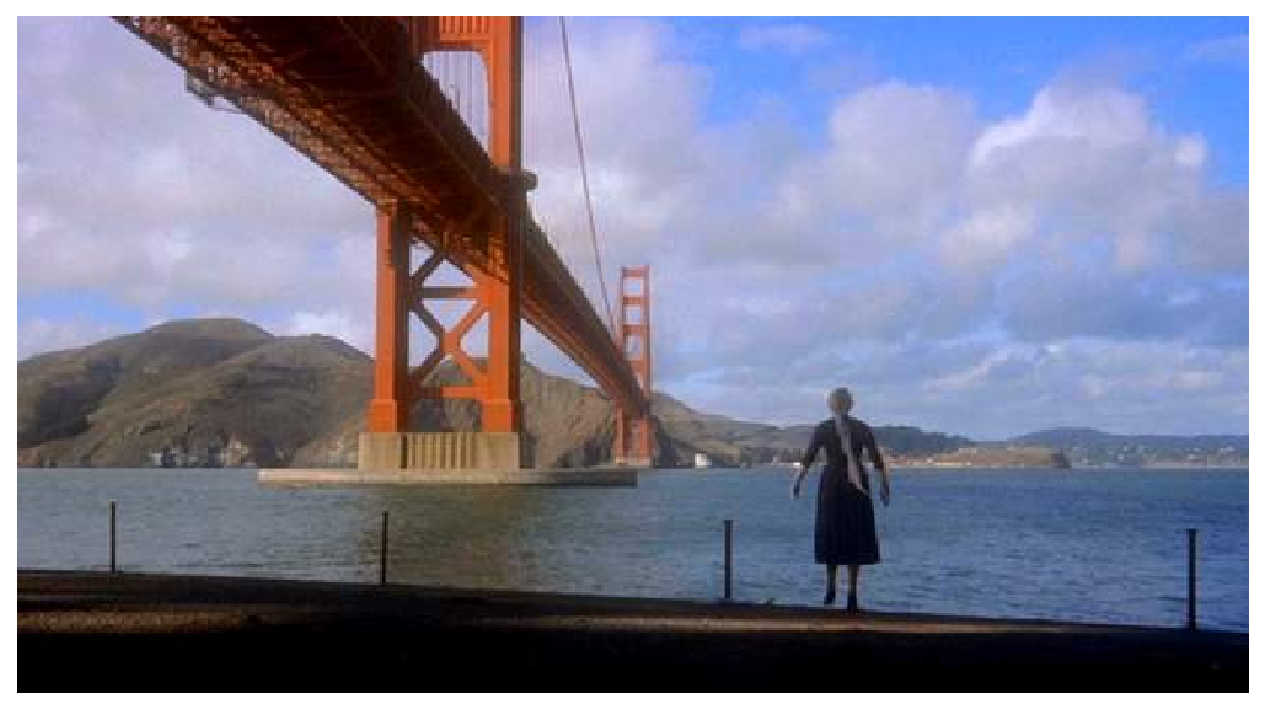
\includegraphics[angle=0,height=0.23\textwidth]{imagens/vertigo.eps} & 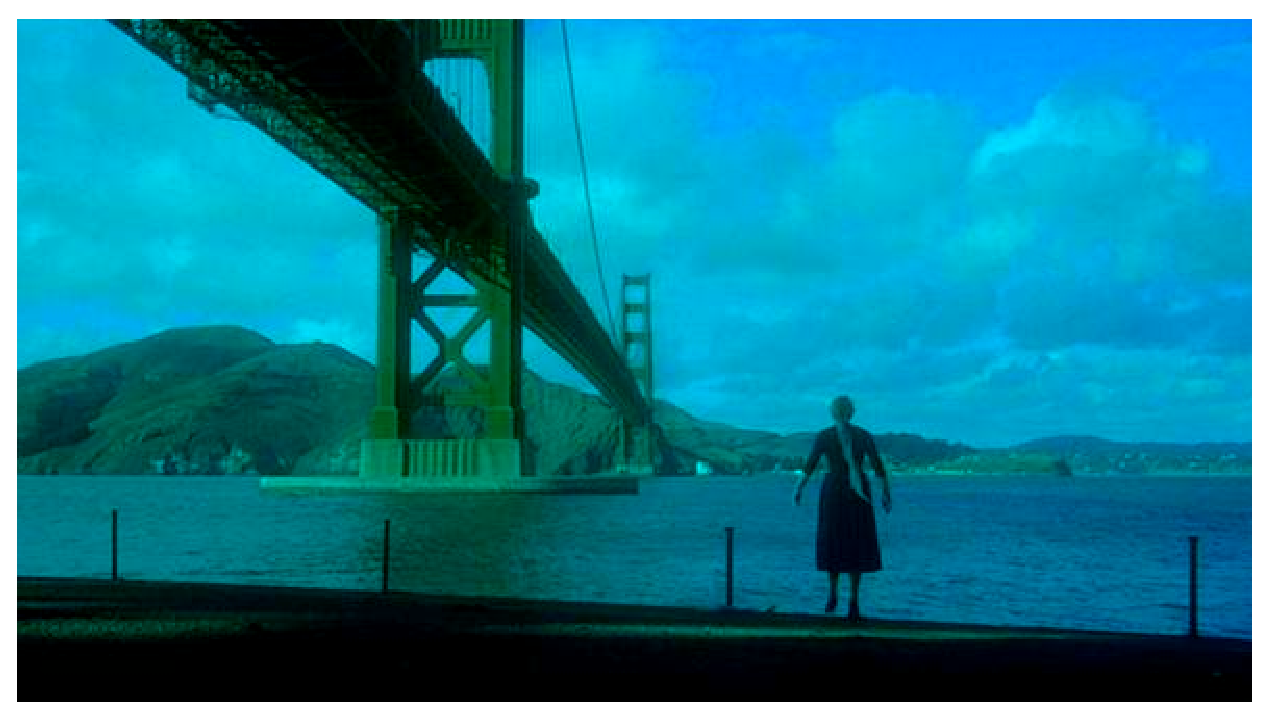
\includegraphics[angle=0,height=0.23\textwidth]{imagens/vertigo_sem_red.eps} \\ \hline \end{tabular}\\\\


\subsection{Cria\c{c}\~{a}o de moldura}

Pretende-se com esta opera\c{c}\~{a}o criar uma moldura preta em redor da imagem. O utilizador deve poder seleccionar a largura da moldura. Note que a imagem original deve ser preservada integralmente, ou seja, nenhum p\'{i}xel da imagem original deve ser descartado ao introduzir a moldura. No exemplo seguinte a imagem original foi modificada atrav\'{e}s da introdu\c{c}\~{a}o de uma moldura com 5 pixeis de largura:\\


\begin{tabular}{|c|c|} \hline Imagem original & Imagem com moldura (5 pixeis)\\ 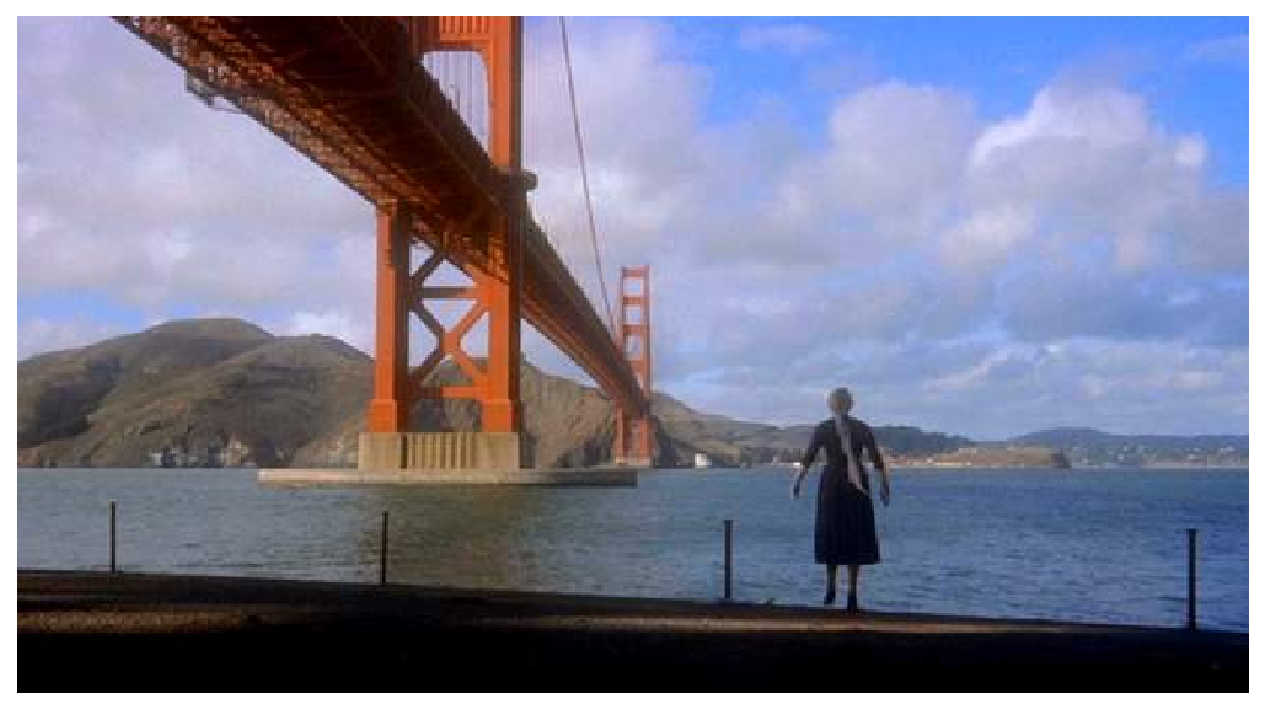
\includegraphics[angle=0,height=0.23\textwidth]{imagens/vertigo.eps} & 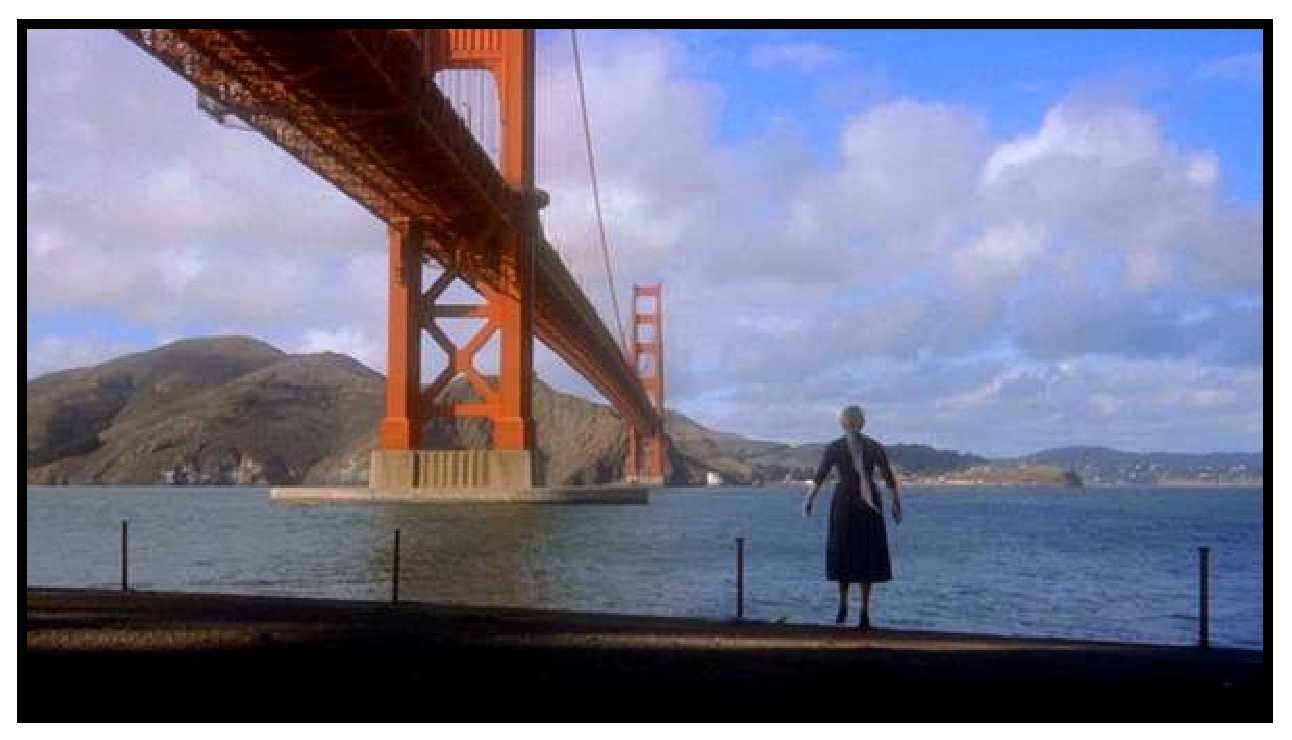
\includegraphics[angle=0,height=0.235\textwidth]{imagens/vertigo_moldura.eps} \\ \hline \end{tabular}\\\\


\subsection{Passagem a tons de cinza}

Uma imagem em tons de cinza pode ser definida como uma imagem que tem valores iguais nas componentes vermelha, azul e verde de cada  p\'{i}xel . Esta opera\c{c}\~{a}o dever\'{a} permitir a convers\~{a}o de uma imagem a cores numa imagem em tons de cinza. Esta opera\c{c}\~{a}o pode ser implementada substituindo cada p\'{i}xel por outro calculado a partir da m\'{e}dia dos valores do p\'{i}xel original. No exemplo seguinte a imagem original foi modificada atrav\'{e}s da sua passagem a tons de cinza:\\

\begin{tabular}{|c|c|} \hline Imagem original & Imagem em tons de cinza \\ 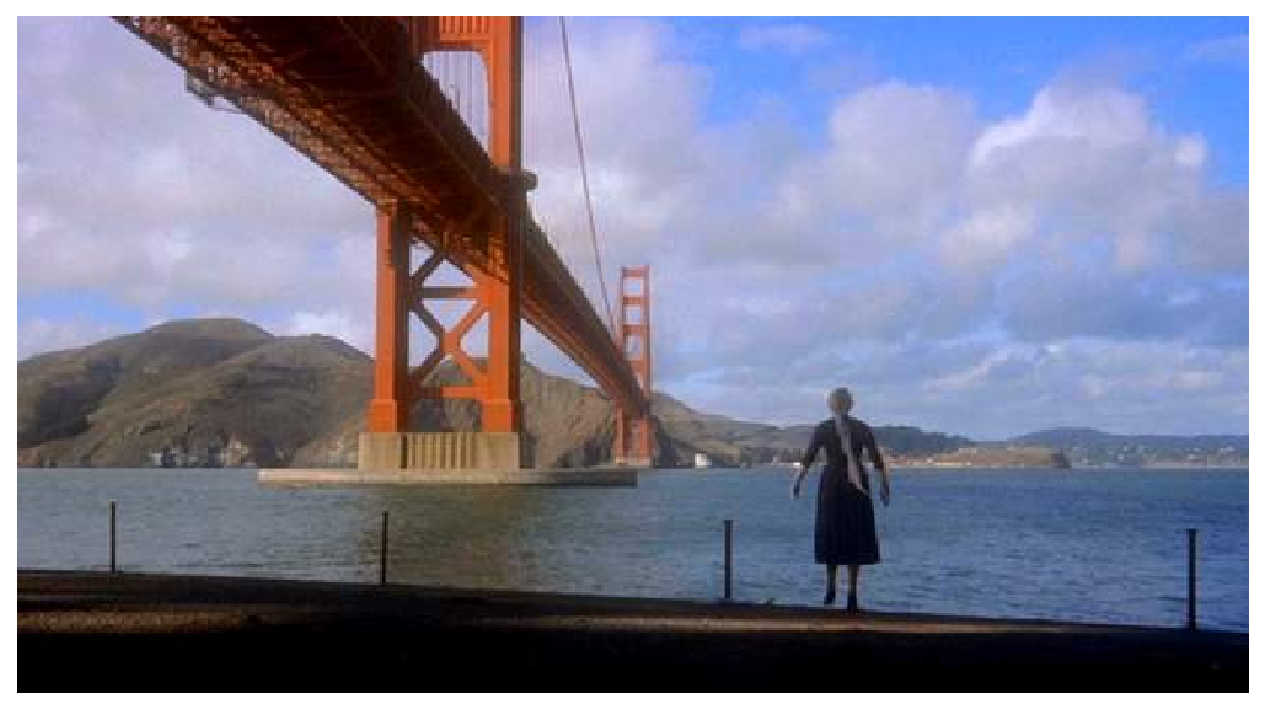
\includegraphics[angle=0,height=0.23\textwidth]{imagens/vertigo.eps} & 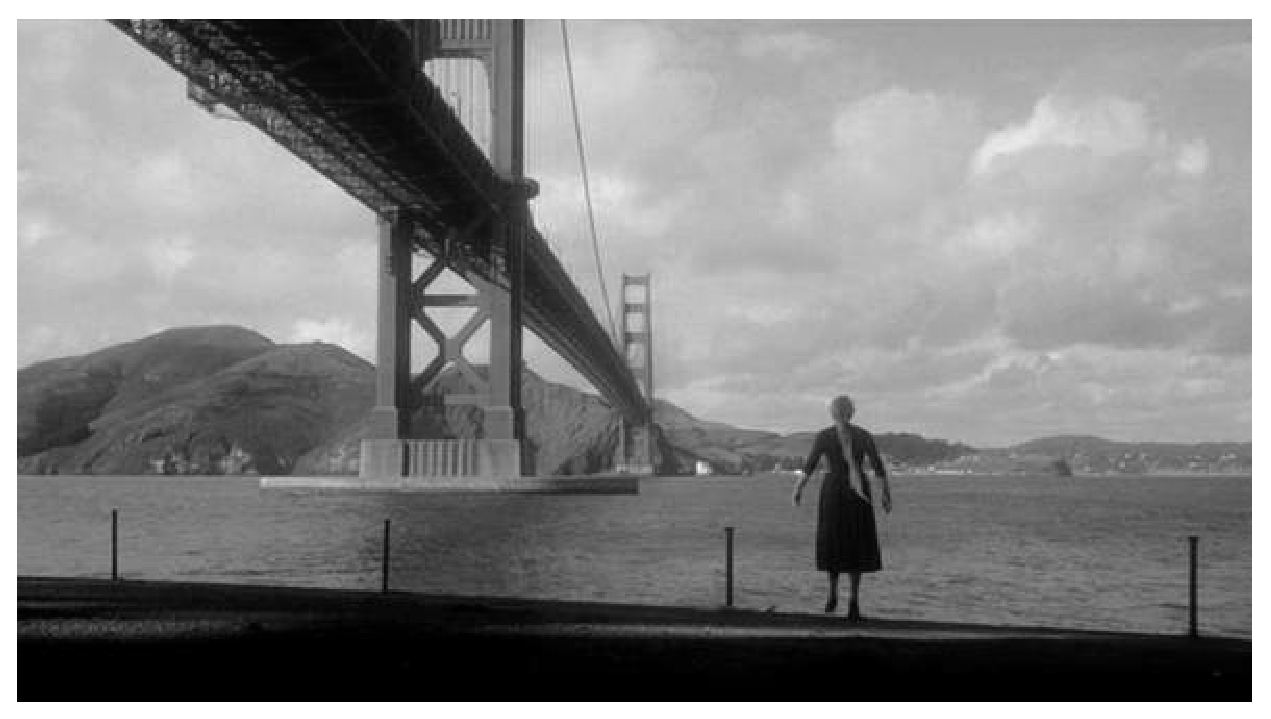
\includegraphics[angle=0,height=0.23\textwidth]{imagens/vertigo_cinza.eps} \\ \hline \end{tabular}\\\\


\subsection{ Rota\c{c}\~{a}o da imagem}

O programa dever\'{a} permitir rodar a imagem original 90, 180 ou 270 graus, de acordo com o sentido de rota\c{c}\~{a}o indicado pelo utilizador (sentido dos ponteiros do rel\'{o}gio ou em sentido inverso). No exemplo seguinte a imagem original � rodada 180 graus:\\\\

\begin{tabular}{|c|c|} \hline Imagem original & Imagem rodada 180 graus \\ 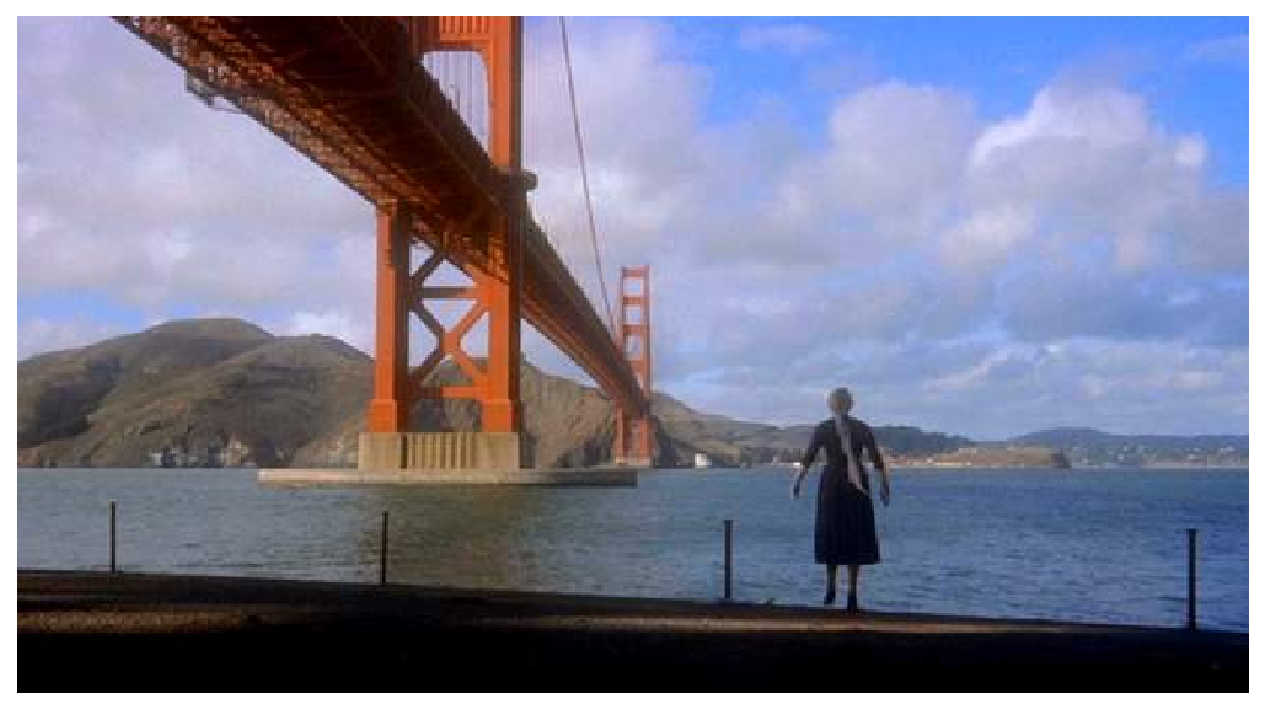
\includegraphics[angle=0,height=0.23\textwidth]{imagens/vertigo.eps} & 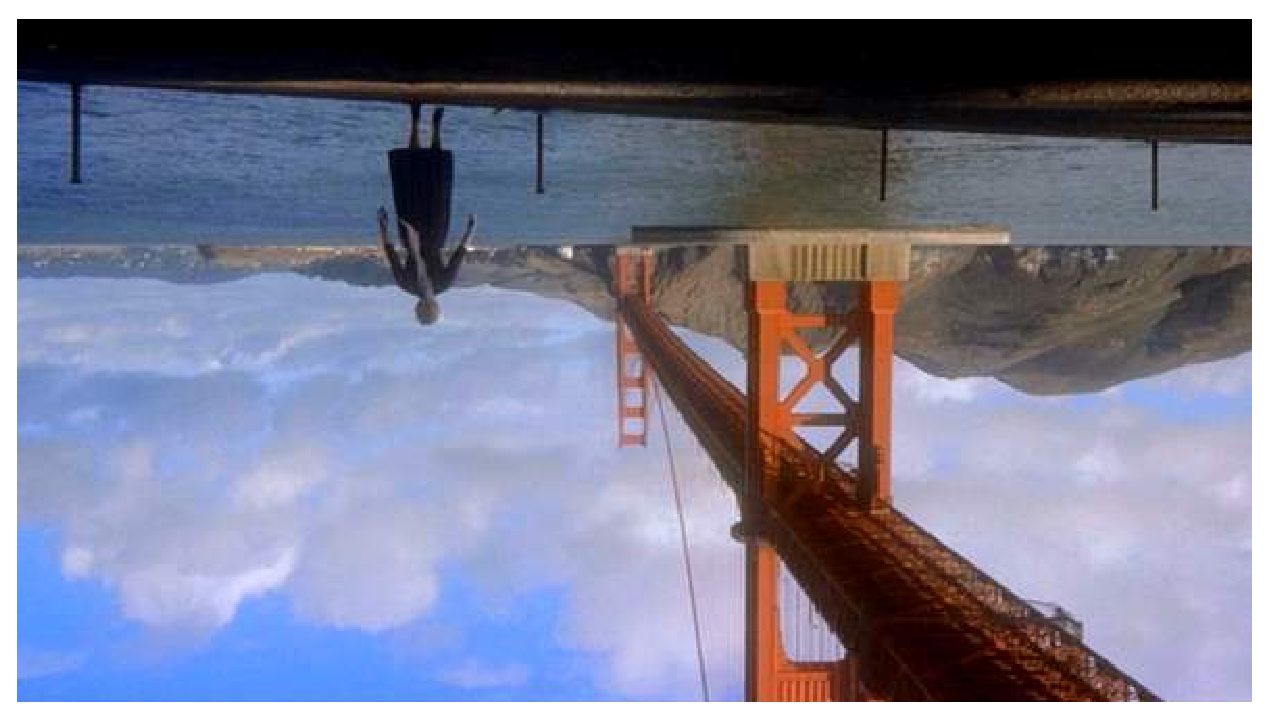
\includegraphics[angle=0,height=0.23\textwidth]{imagens/vertigo_rot180.eps} \\ \hline \end{tabular}\\\\



\subsection{Reflex\~{a}o de imagem}

O programa dever\'{a} permitir reflectir horizontal ou verticalmente uma imagem. No exemplo seguinte a nova imagem \'{e} obtida por reflex\~{a}o horizontal da imagem original:\\\\

\begin{tabular}{|c|c|} \hline Imagem original & Reflex\~{a}o horizontal da imagem \\ 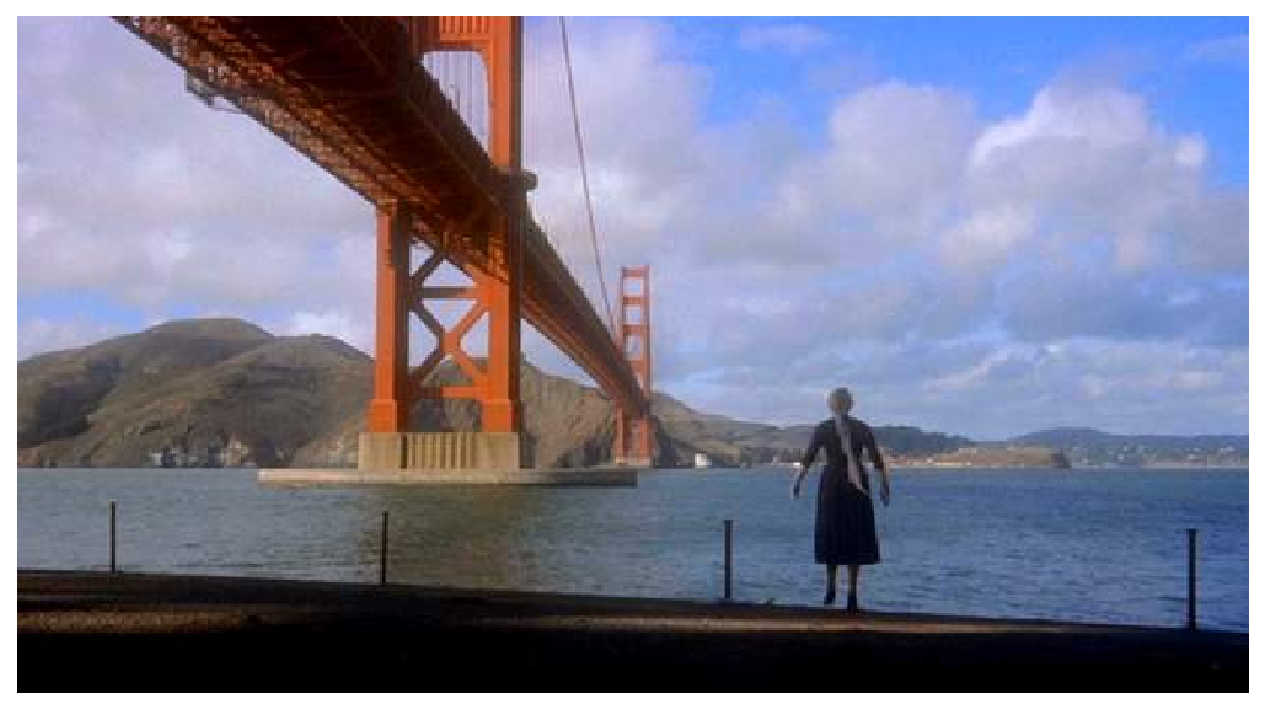
\includegraphics[angle=0,height=0.23\textwidth]{imagens/vertigo.eps} & \includegraphics[angle=0,height=0.23\textwidth]{imagens/vertigo_mirror_hor.eps} \\ \hline \end{tabular}\\\\


\subsection{Corte de imagem}

O corte de uma imagem com o objectivo de seleccionar uma \'{a}rea de interesse \'{e} uma opera\c{c}\~{a}o frequentemente utilizada nos programas de tratamento de imagens. Pretende-se desta forma permitir que o utilizador possa cortar a imagem original, de acordo com uma regi\~{a}o seleccionada. O utilizador dever\'{a} seleccionar a zona da imagem a preservar indicando as coordenadas dos p\'{i}xeis correspondentes aos cantos superior esquerdo e inferior direito dessa zona na imagem original. No exemplo seguinte a imagem final foi obtida por corte da imagem original, seleccionando como imagem pretendida a zona na imagem original definida pelas coordenadas 200,200 (coordenadas do p\'{i}xel no canto superior esquerdo) e 500,10 (coordenadas do p\'{i}xel no canto inferior direito):\\\\

\begin{tabular}{|c|c|} \hline Imagem original & Imagem obtida por corte\\ 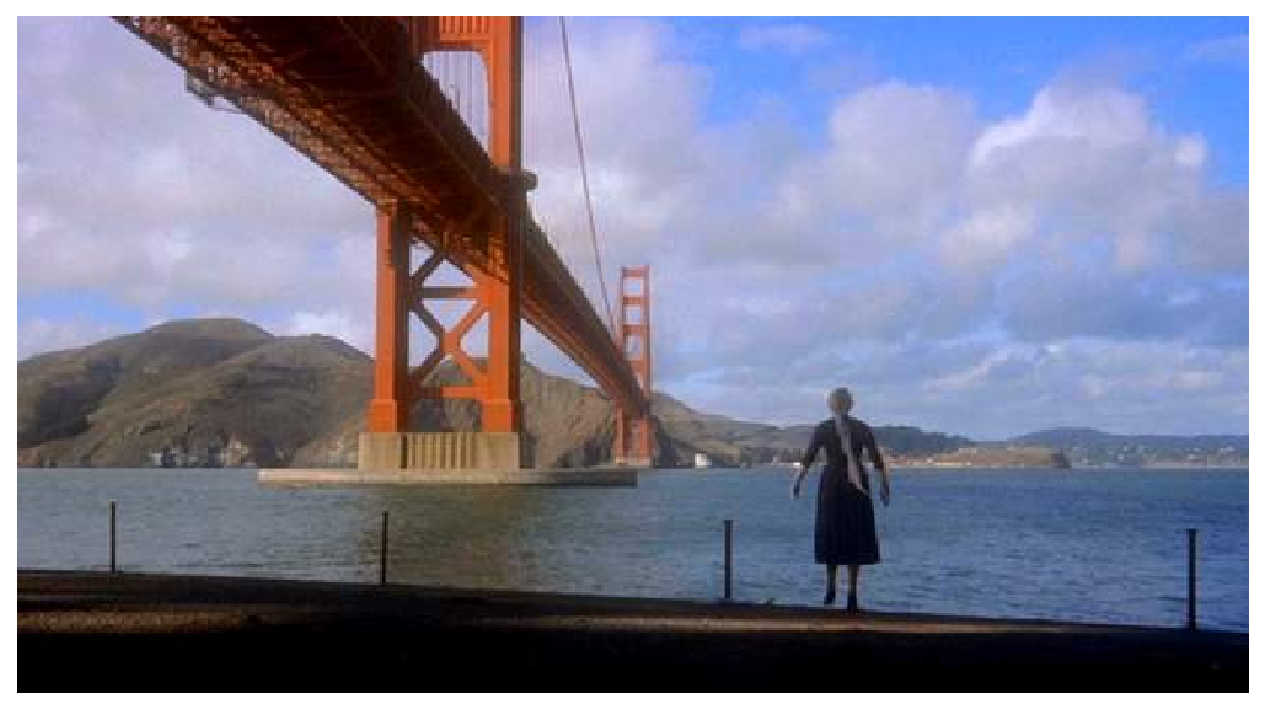
\includegraphics[angle=0,height=0.23\textwidth]{imagens/vertigo.eps} & 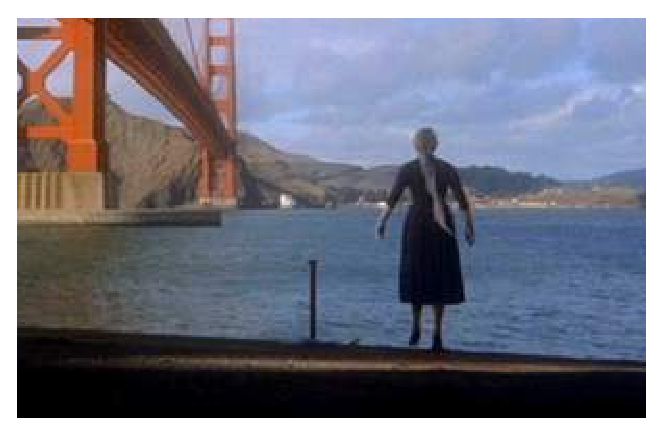
\includegraphics[angle=0,height=0.17\textwidth]{imagens/vertigo_cortada.eps} \\ \hline \end{tabular}\\\\


\subsection{Negativo de imagem}

O negativo de uma imagem pode na pr\'{a}tica ser obtido calculando o negativo dos 3 componentes de cor que definem cada p\'{i}xel da imagem. No exemplo seguinte a imagem original foi modificada atrav\'{e}s da sua passagem a negativo:\\

\begin{tabular}{|c|c|} \hline Imagem original & Negativo da imagem\\ 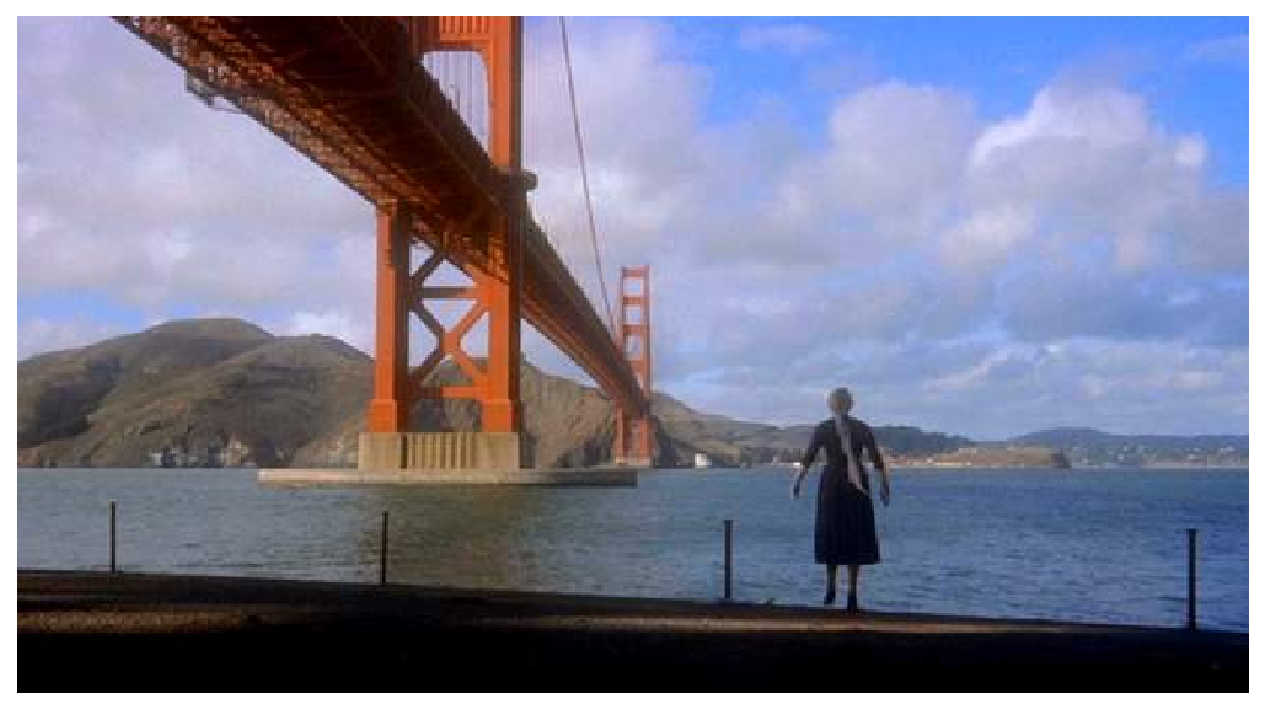
\includegraphics[angle=0,height=0.23\textwidth]{imagens/vertigo.eps} & 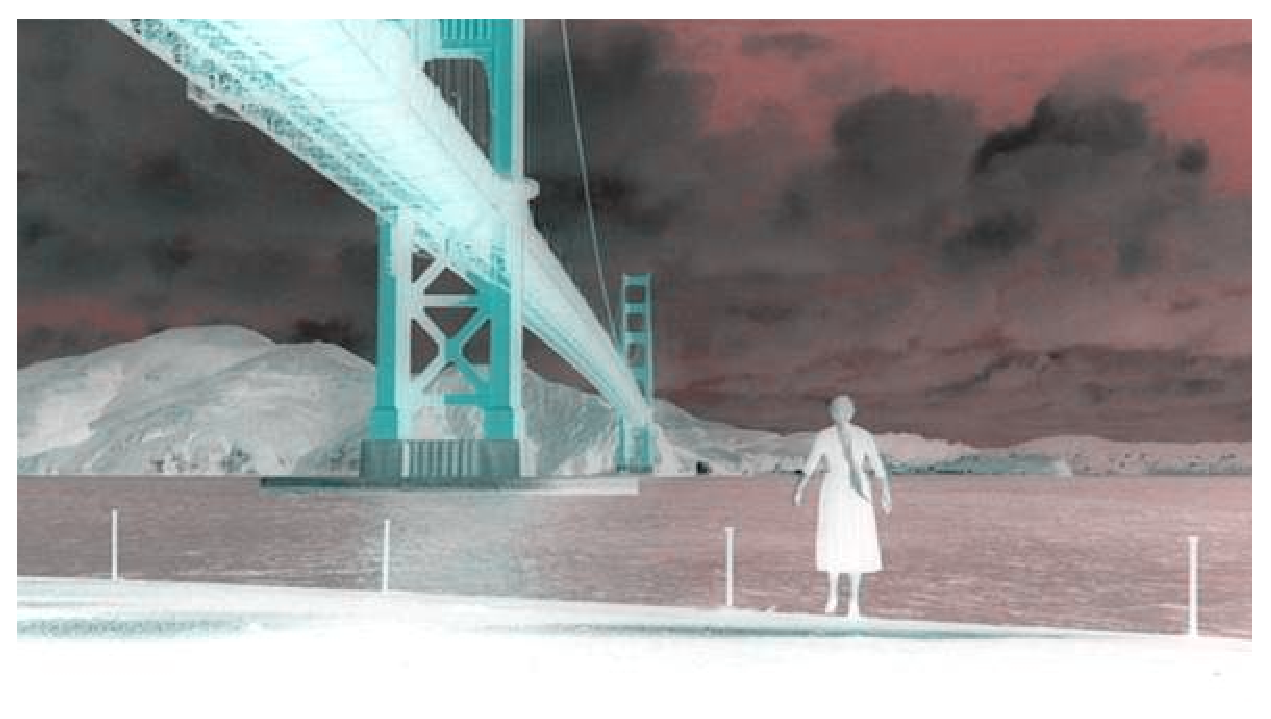
\includegraphics[angle=0,height=0.23\textwidth]{imagens/vertigo_neg.eps} \\ \hline \end{tabular}\\\\


\section{Outras opera\c{c}\~{o}es de processamento de imagem}


\subsection{Esteganografia}\label{sec:extra}

As t\'{e}cnicas de esteganografia permitem em geral ocultar informa\c{c}\~{a}o considerada secreta, utilizando para o efeito mensagens aparentemente in\'{o}cuas. Os dados que descrevem uma determinada imagem podem igualmente ser manipulados no sentido de ocultar uma mensagem secreta, de forma totalmente transparente. Pretende-se portanto que o programa ofere\c{c}a uma opc\c{c}\~{a}o para ocultar uma mensagem de texto num ficheiro de imagem, ou em alternativa ler uma mensagem secreta armazenada de forma oculta num ficheiro de imagem.

A t\'{e}cnica a utilizar para ocultar uma mensagem secreta passa por utilizar os bits menos significativos de cada p\'{i}xel (ou das 3 componentes de cor do p\'{i}xel) para armazenar a mensagem. De facto,  \'{e} poss\'{i}vel verificar que a mudan\c{c}a dos bits menos significativos de cada componente de cor ou p\'{i}xel afectam muito pouco a imagem final, o mesmo n\~{a}o podendo ser dito dos bits mais significativos. Se for alterado apenas o bit menos significativo em cada componente de cor ou p\'{i}xel da imagem, \'{e} de facto muito dif\'{i}cil ou mesmo imposs\'{i}vel distinguir a imagem alterada da original. Por exemplo, \'{e} muito dif\'{i}cil distinguir entre os p\'{i}xeis com o valor 10000000 (128 em decimal) e 10000001 (129 em decimal). J\'{a} altera\c{c}\~{o}es a bits mais significativos s\~{a}o facilmente percept\'{i}veis. Por exemplo, a diferen\c{c}a entre os valores 00001000 (8 em decimal) e 10001000 (136 em decimal) j\'{a} \'{e} percept\'{i}vel.

A t\'{e}cnica a implementar consistir\'{a} portanto na altera\c{c}\~{a}o do bit menos significativo de cada componente de cor (RGB) de cada p\'{i}xel da imagem original, em tantos p\'{i}xeis quantos os necess\'{a}rios para armazenar a informa\c{c}\~{a}o secreta. Considerando que a informa\c{c}\~{a}o secreta consiste numa string, o que se pretende \'{e} ocultar cada um dos 8 bits que formam cada caracter na imagem, utilizando para o efeito o bit menos significativo de cada componente de cor dos p\'{i}xeis. O exemplo seguinte ilustra o armazenamento dos primeiros dois caracteres da string "IPRP" num ficheiro de imagem:  \\

\begin{tabular}{|c|c|c|}
\hline Caracter a ocultar & Componentes RGB originais & Componentes RGB modificados \\ 

\hline ... & ... & ... \\

\hline I ({\bf01001001}) &

\begin{tabular}{|c|c|}
\hline R & 01100111 \\ 
\hline G & 01011010 \\
\hline B & 10001101 \\
\hline R & 10100111 \\ 
\hline G & 01011010 \\
\hline B & 10101101 \\
\hline R & 11001010 \\ 
\hline G & 10011011 \\
\hline 
\end{tabular} &

\begin{tabular}{|c|c|}
\hline R & 0110011{\bf0} \\ 
\hline G & 0101101{\bf1} \\
\hline B & 1000110{\bf0} \\
\hline R & 1010011{\bf0} \\ 
\hline G & 0101101{\bf1} \\
\hline B & 1010110{\bf0} \\
\hline R & 1100101{\bf0} \\ 
\hline G & 1001101{\bf1} \\
\hline 
\end{tabular} \\

\hline P ({\bf01010000}) & 

\begin{tabular}{|c|c|}
\hline B & 01010111 \\ 
\hline R & 10101010 \\
\hline G & 11101101 \\
\hline B & 10100101 \\ 
\hline R & 01111010 \\
\hline G & 00101101 \\
\hline B & 11011010 \\ 
\hline R & 10101001 \\
\hline 
\end{tabular} &

\begin{tabular}{|c|c|}
\hline B & 0101011{\bf0} \\ 
\hline R & 1010101{\bf1} \\
\hline G & 1110110{\bf0} \\
\hline B & 1010010{\bf1} \\ 
\hline R & 0111101{\bf0} \\
\hline G & 0010110{\bf0} \\
\hline B & 1101101{\bf0} \\ 
\hline R & 1010100{\bf0} \\
\hline 
\end{tabular} \\

\hline ... & ... & ... \\

\hline 
\end{tabular}\\\\


Tal como o exemplo anterior ilustra, o c\'{o}digo ASCII de cada caracter \'{e} armazenado nas componentes RGB da imagem, utilizando para o efeito o bit menos significativo de cada componente. O armazenamento \'{e} sequencial, ou seja, o primeiro do bit do caracter seguinte come\c{c}a na componente imediatamente a seguir \`{a} ultima componente de cor utilizada para armazenar o \'{u}ltimo bit do caracter anterior. Por \'{u}ltimo, refira-se que o programa dever\'{a} ser capaz de determinar se um determinado ficheiro de imagem disp\~{o}em ou n\~{a}o de uma mensagem secreta armazenada.  
\\


\subsection{Encripta\c{c}\~{a}o}

O objectivo desta opera\c{c}\~{a}o \'{e} proteger uma imagem considerada confidencial, utilizando para o efeito um algor\'{i}tmo de encripta\c{c}\~{a}o, que iremos utilizar para encriptar ou desencriptar uma imagem. Embora existam in\'{u}meros algor\'{i}tmos de encripta\c{c}\~{a}o em uso actualmente, o nosso prop\'{o}sito passa apenas por poder modificar a imagem de modo a torn\'{a}-la impercept\'{i}vel quando comparada com a imagem original. Como tal, iremos implementar um algor\'{i}tmo bastante simples, que passamos a descrever.

A opera\c{c}\~{a}o de encripta\c{c}\~{a}o implementada pelo nosso algoritmo consiste em trocar a ordem \`{a}s colunas da imagem original. Para que tal seja poss\'{i}vel, o algor\'{i}tmo deve dispor de informa\c{c}\~{a}o secreta que indique qual a nova ordem de cada coluna na imagem encriptada, relativamente \`{a} imagem original. Esta informa\c{c}\~{a}o secreta consistir\'{a} numa s\'{e}rie de n\'{u}meros, de dimens\~{a}o igual \`{a} dimens\~{a}o horizontal da imagem, para que todas as colunas possam ser trocadas.

A s\'{e}rie de n\'{u}meros representativa da nova ordem das colunas na imagem encriptada dever\'{a} ser uma s\'{e}rie pseudo-aleatoria gerada pelo programa, com recurso \`{a}s fun\c{c}\~{o}es do m\'{o}dulo \textit{random} do Python. Para que seja poss\'{i}vel utilizar s\'{e}ries pseudo-aleat\'{o}rias diferentes, o programa dever\'{a} solicitar uma password ao utilizador e derivar a semente inicial de gera\c{c}\~{a}o de n\'{u}meros aleat\'{o}rios a partir dessa password. O programa deve somar o c\'{o}digo ASCII de todos os caracteres que constituem a password pedida ao utilizador, e utilizar o valor resultante como semente no processo de gera\c{c}\~{a}o de n\'{u}meros aleat\'{o}rios. O exemplo seguinte ilustra o resultado da encripta\c{c}\~{a}o de uma imagem utilizando a password "IPRP": \\


\begin{tabular}{|c|c|} \hline Imagem original & Imagem encriptada\\ 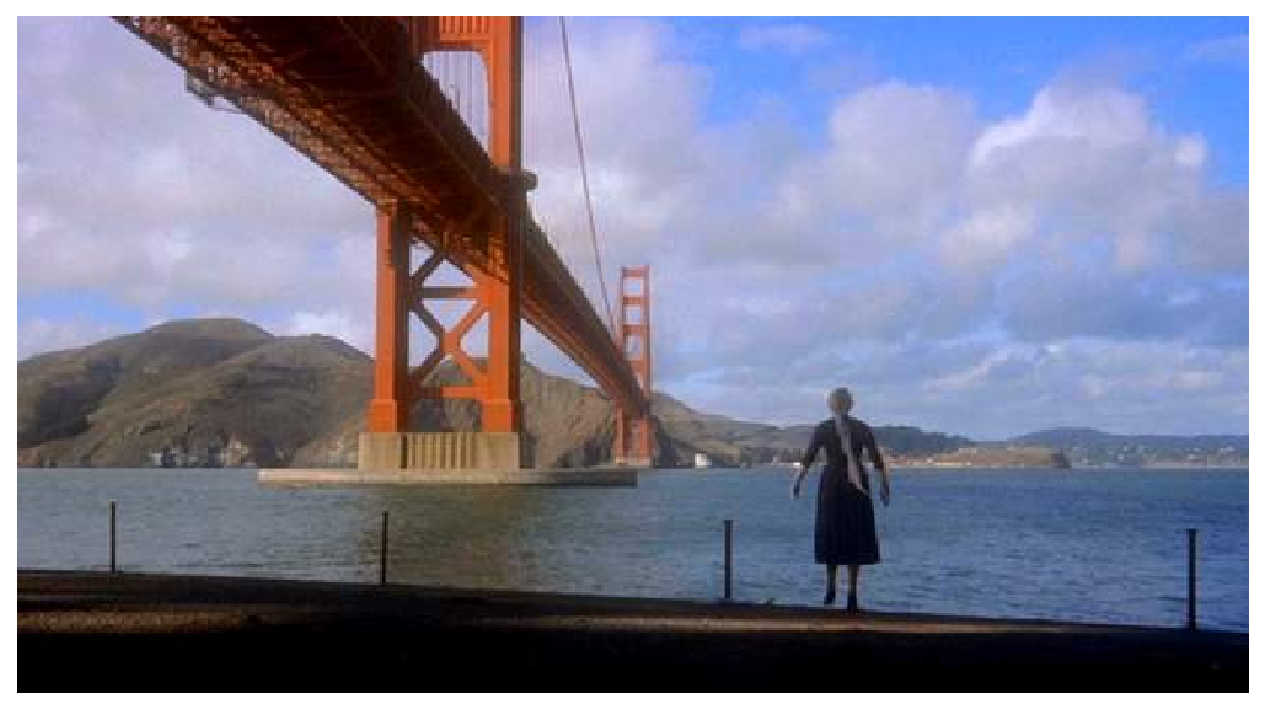
\includegraphics[angle=0,height=0.23\textwidth]{imagens/vertigo.eps} & 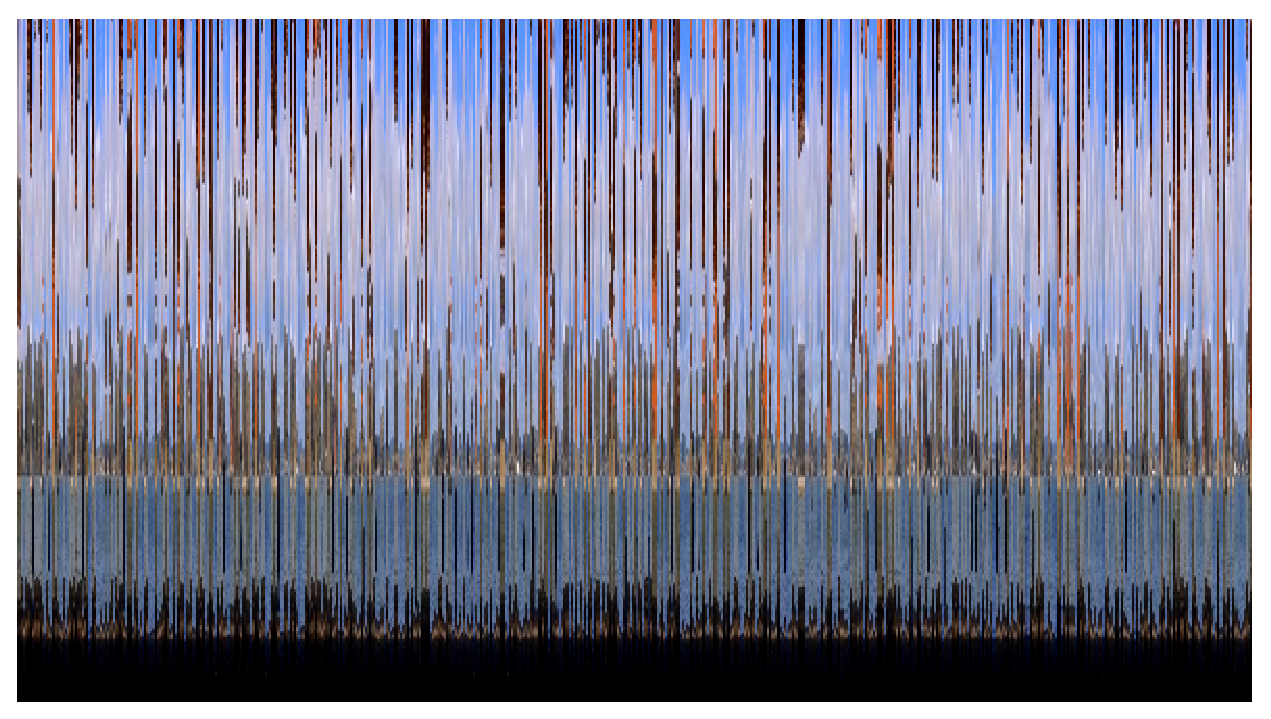
\includegraphics[angle=0,height=0.23\textwidth]{imagens/vertigo_encriptada.eps} \\ \hline \end{tabular}\\\\

O processo de desencripta\c{c}\~{a}o decorrer\'{a} de forma inversa, ou seja, considerando o n\'{u}mero de ordem de cada coluna a repor para obter novamente a imagem inicial, de acordo com os valores da s\'{e}rie de n\'{u}meros pseudo-aleat\'{o}rios gerada utilizando a mesma password.\\


\section{Regras, crit\'{e}rios e m\'{e}todos de avalia\c{c}\~{a}o}


\subsection{Constitui\c{c}\~{a}o de grupos de trabalho}

O presente trabalho deve ser executado em grupos de 2 alunos. Em situa\c{c}\~{a}o alguma ser\~{a}o aceites grupos com mais do que 2 alunos. Excepcionalmente, e apenas em casos bem fundamentados, se aceitar�o trabalhos individuais.\\\


\subsection{Metas de avalia\c{c}\~{a}o}

A metas de avalia\c{c}\~{a}o s\~{a}o obrigat\'{o}rias e os seus objectivos s\~{a}o descritos a seguir:\\


\begin{tabular}{|p{14.5cm}|}
\hline 

{\bf META 1}:\\
O programa dever\'{a} apresentar as seguintes funcionalidades (ver sec\c c�o \ref{sec:gerais}):\\\\

{\bf a}. Leitura de imagem a partir de ficheiro para estrutura de dados em mem\'{o}ria. O utilizador dever\'{a} poder indicar o nome do ficheiro pretendido.\\\\

{\bf b}. Utilizando as fun\c{c}\~{o}es j\'{a} referidas da PIL, o programa dever\'{a} apresentar a imagem numa janela.\\\\

{\bf c}. Armazenamento da mesma imagem noutro ficheiro, novamente de acordo com nome indicado pelo utilizador.\\

\hline 

{\bf META 2}:\\
O programa dever\'{a} apresentar as seguintes funcionalidades (ver sec\c c�o \ref{sec:funda}):\\\\


{\bf a}. Apresenta\c{c}\~{a}o do menu com as opc\c{c}\~{o}es suportadas pelo programa, bem como a leitura da opc\c{c}\~{a}o seleccionada pelo utilizador.\\\\

{\bf b}. Tratamento da imagem com as  opera\c{c}\~{o}es fundamentais de processamento de imagens descritas anteriormente.\\\\

\hline 

{\bf META 3}:\\
Entrega e defesa do trabalho, na sua vers\~{a}o final e implementando todas as opera\c{c}\~{o}es descritas anteriormente (ver as sec\c c�es \ref{sec:gerais}, \ref{sec:funda} e \ref{sec:extra}).\\\\

\hline 
\end{tabular}\\


Nota: Factores que podem valorizar o seu programa incluem: optimiza\c{c}\~{a}o do desempenho das opera\c{c}\~{o}es de processamento de imagens, tratamento de excep\c{c}\~{o}es;\\


{\color{red}{\Huge \bf Note Bem} }
\begin{enumerate}
\item N�o cumprir a Meta 1 ou entregar fora do prazo faz perder 20\% da nota;
\item N�o cumprir a Meta 2 ou entregar fora do prazo faz perder 30\% da nota;
\item N�o cumprir a Meta 3 implica reprova\c c�o na cadeira.
\item A fraude denota uma grave falta de \'{e}tica e constitui um comportamento n\~{a}o admiss\'{i}vel num estudante do ensino superior e futuro profissional licenciado. Qualquer tentativa de fraude na elabora\c{c}\~{a}o do presente Trabalho Pr\'{a}tico conduzir\'{a} inevit\'{a}velmente \`{a} reprova\c{c}\~{a}o imediata na cadeira
\end{enumerate}



\end{document}
